\chapter{گراف}
\thispagestyle{empty}

\section{آشنایی با گراف‌ها}
گراف $G$ زوجی مرتب چون
$G(V,E)$
است که در آن $V$ مجموعه‌ای متناهی و ناتهی است و $E$ زیرمجموعه‌ای از مجموعه‌ی تمام زیرمجموعه‌های دوعضوی $V$ است. اعضای $V$ را رأس‌های $G$ و اعضای $E$ را یال‌های $G$ می‌نامیم. مجموعه‌ی رأس‌های $G$ را با
$V(G)$
و مجموعه‌ی یال‌های آن را با
$E(G)$
نمایش می‌دهیم.
\begin{example}
	اگر
	$V=\{a,b,c,d,e\}$
	و
	$E=\left\{\{a,d\},\{b,c\},\{b,e\}\right\}$
	آنگاه
	$G=(V,E)$
	گرافی است که پنج رأس و سه یال دارد.
\end{example}

\textbf{دو رأس مجاور (همسایه):}
اگر در گراف $G$،
$u,v \in V(G)$
و
$\{u,v\} \in E(G)$،
برای سادگی، به جای
$\{u,v\}$
می‌نویسیم $uv$ و می‌گوییم دو رأس $u$ و $v$ مجاور (همسایه) هستند. در این صورت گاهی گفته می‌شود رأس $u$ (همچنین رأس $v$) بر یال $uv$ واقع است. اصطلاح رایج دیگر این است که در $G$ یال $uv$ از رأس $u$ (همچنین از رأس $v$) می‌گذرد. رأس‌های $u$ و $v$ دو سر یال $uv$ نام دارند.
\begin{example}
	اگر
	$V=\{a,b,c,d,e\}$
	و
	$E=\{ab,ac,ae,bd,cd,ce,de\}$
	آنگاه
	$G(V,E)$
	گرافی است که پنج رأس و هفت یال دارد. دو رأس $a$ و $b$ مجاورند زیرا
	$ab \in E$
	ولی دو رأس $b$ و $e$ مجاور نیستند چون
	$be \notin E$.
	از رأس $a$ سه یال و از رأس $b$ دو یال می‌گذرد.
\end{example}

هر گراف را می‌توان با یک نمودار، موسوم به نمودار گراف، نمایش داد. برای رسم نمودار یک گراف روش یکتایی مدنظر نیست. آنچه مهم است این است که باید مشخص باشد که گراف موردنظر چند رأس و چند یال دارد و کدام یال به کدام رأس‌ها متصل است.
\begin{example}
	اگر
	$V(G)=\{a,b,c,d\}$
	و
	$E(G)=\{ab,ac,bd\}$
	آنگاه $G$ گرافی است که چهار رأس و سه یال دارد. سه نمودار از این گراف را در شکل‌های زیر رسم کرده‌ایم.
	\begin{figure}[H]
		\centering
		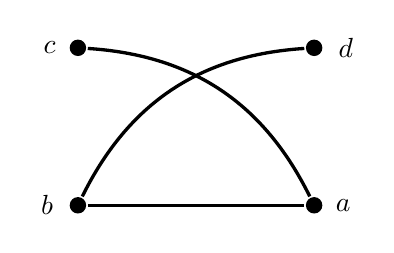
\begin{tikzpicture}[every node/.style={circle, fill=black, inner sep=2.1pt, scale=1}, every path/.style={line width=1.2pt}]
			\node[label=left:$c$] (c) at (0,2) {};
			\node[label=right:$d$] (d) at (3,2) {};
			\node[label=left:$b$] (b) at (0,0) {};
			\node[label=right:$a$] (a) at (3,0) {};
			\draw (b)--(a);
			\draw[bend left=30] (b) to (d);
			\draw[bend left=30] (c) to (a);
		\end{tikzpicture}
		\hspace{2cm}
		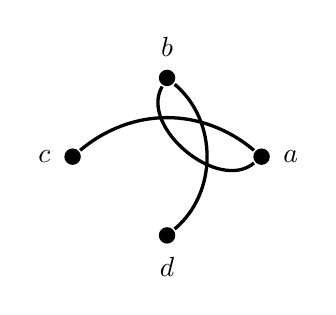
\begin{tikzpicture}[every node/.style={circle, fill=black, inner sep=2.1pt, scale=1}, every path/.style={line width=1.2pt}]
			\node[label=above:$b$] (b) at (0,2) {};
			\node[label=left:$c$] (c) at (-1.2,1) {};
			\node[label=right:$a$] (a) at (1.2,1) {};
			\node[label=below:$d$] (d) at (0,0) {};
			\draw (b) to[out=-120, in=220] (a);
			\draw (c) to[out=40, in=140] (a);
			\draw (b) to[out=-40, in=40] (d);
		\end{tikzpicture}
		\hspace{2cm}
		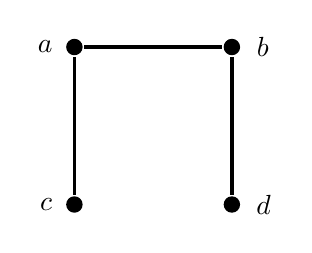
\begin{tikzpicture}[every node/.style={circle, fill=black, inner sep=2.1pt, scale=1}, every path/.style={line width=1.2pt}]
			\node[label=left:$a$] (a) at (0,2) {};
			\node[label=right:$b$] (b) at (2,2) {};
			\node[label=left:$c$] (c) at (0,0) {};
			\node[label=right:$d$] (d) at (2,0) {};
			\draw (a)--(b);
			\draw (a)--(c);
			\draw (b)--(d);
		\end{tikzpicture}
	\end{figure}
\end{example}

ممکن است بین دو رأس از یک گراف، بیش از یک یال وجود داشته باشد. همچنین یک یال ممکن است یک رأس را به خود آن رأس وصل نماید که در این صورت به این یال طوقه (حلقه) گفته می‌شود. گرافی را که در آن هیچ یک از این دو مورد اتفاق نیفتاده باشد، گراف ساده می‌گوییم. ما در این فصل، فقط گراف‌های ساده را بررسی می‌کنیم و منظورمان از گراف، گراف ساده است.

\begin{example}
	گراف‌های زیر، گراف ساده نیستند، بلکه مالتی‌گراف هستند.
	\begin{figure}[H]
		\centering
		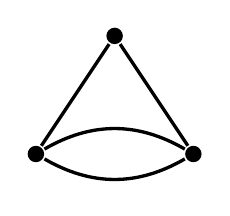
\begin{tikzpicture}[every node/.style={circle, fill=black, inner sep=2.1pt, scale=1}, every path/.style={line width=1.2pt}]
			\node (a) at (1,1.5) {};
			\node (b) at (0,0) {};
			\node (c) at (2,0) {};
			\draw (b) to[out=30, in=150] (c);
			\draw (b) to[out=-30, in=-150] (c);
			\draw (a)--(b);
			\draw (a)--(c);
		\end{tikzpicture}
		\hspace{2cm}
		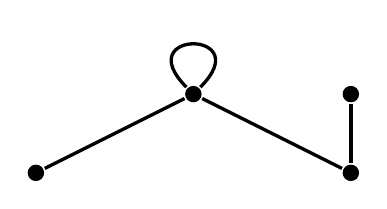
\begin{tikzpicture}[every node/.style={circle, fill=black, inner sep=2.1pt, scale=1}, every path/.style={line width=1.2pt}]
			\node (a) at (0,0) {};
			\node (b) at (2,1) {};
			\node (c) at (4,0) {};
			\node (d) at (4,1) {};
			\draw (a)--(b);
			\draw (b)--(c);
			\draw (c)--(d);
			\draw[loop, looseness=15] (b) to (b);
		\end{tikzpicture}
	\end{figure}
\end{example}

می‌دانیم که اگر مجموعه‌ای $p$ عضو داشته باشد
($p \in \mathbb{Z}^+$)،
تعداد زیرمجموعه‌های دو عضوی آن
$\frac{p(p-1)}{2}$
است. بنابراین اگر گرافی $p$ رأس و $q$ یال داشته باشد، داریم:
$$0 \leq q \leq \frac{p(p-1)}{2}$$

\textbf{مرتبه و اندازه‌ی یک گراف:}
در هر گراف
$G(V,E)$
تعداد اعضای مجموعه‌ی $V$ یعنی $|V(G)|$ را مرتبه‌ی $G$ می‌گوییم و با $p(G)$ یا $p$ نمایش می‌دهیم و تعداد اعضای مجموعه‌ی $E$ یعنی $|E(G)|$ را اندازه‌ی $G$ می‌نامیم و با $q(G)$ یا $q$ نمایش می‌دهیم.

\textbf{درجه‌ی یک رأس:}
درجه‌ی رأس $v$ از گراف $G$ برابر با تعداد یال‌هایی از $G$ است که از رأس $v$ می‌گذرند. این عدد را با
$\deg_G(v)$
و گاهی به‌طور ساده با
$\deg(v)$
نمایش می‌دهیم. اگر
$\deg(v)$
عددی فرد باشد، $v$ را یک رأس فرد و اگر عددی زوج باشد $v$ را یک رأس زوج از گراف $G$ می‌نامیم.

\begin{theorem}
	اگر
	$V=\{v_1,v_2,\cdots,v_p\}$
	مجموعه‌ی رأس‌های گراف $G$ با اندازه‌ی $q$ باشد، آنگاه:
	$$\sum_{i=1}^{p}\deg(v_i) = 2q$$
	\textbf{برهان:}
	هر یال تنها دو سر دارد، یعنی دقیقاً از دو رأس $G$ می‌گذرد و لذا در طرف چپ فرمول بالا هر یال دو بار به حساب می‌آید.
	\qed
	\\ \df \\
	\textbf{نتیجه:}
	تعداد رأس‌های فرد هر گراف، زوج است. \\
	\textbf{برهان:}
\end{theorem}

\textbf{گراف $k$-منتظم:}
گرافی را که درجه‌ی تمام رأس‌های آن با هم مساوی و برابر با عدد $k$ باشند، گراف $k$-منتظم می‌نامیم.

\textbf{رأس تنها و گراف تهی:}
به رأسی که درجه‌ی آن صفر باشد؛ یعنی هیچ یالی به آن متصل نباشد، رأس تنها (ایزوله) می‌گوییم. گرافی را که تمام رأس‌های آن تنها باشند، گراف تهی می‌نامیم.

\textbf{مجموعه‌ی همسایه‌های یک رأس:}
فرض کنیم
$v \in V(G)$.
به مجموعه‌ی رأس‌هایی از گراف $G$ که به رأس $v$ متصل هستند، «همسایگی باز رأس $v$» می‌گوییم و با
$N_G(v)$
نمایش می‌دهیم. اضافه کردن خود رأس $v$ به
$N_G(v)$
«همسایگی بسته‌ی رأس $v$» را به دست می‌دهد که آن را با
$N_G[v]$
نمایش می‌دهیم.
$$N_G(v)=\{u \in V(G) : uv \in E(G)\}$$
$$N_G[v]=N_G(v) \cup \{v\}$$

\textbf{دو یال مجاور:}
دو یال را مجاور گوییم هرگاه رأسی وجود داشته باشد که هر دوی آن‌ها به آن متصل باشند.

\textbf{بزرگ‌ترین و کوچک‌ترین درجه‌ی یک گراف:}
بزرگ‌ترین عدد در بین درجه‌های رأس‌های گراف $G$ را با
$\Delta(G)$
و کوچک‌ترین آن‌ها را با
$\delta(G)$
نمایش می‌دهیم و به ترتیب آن‌ها را مکسیمم و مینیمم درجه‌ی گراف می‌نامیم.

\textbf{زیرگراف:}
یک زیرگراف از $G$ گرافی است که مجموعه‌ی رأس‌های آن زیرمجموعه‌ای از مجموعه‌ی رأس‌های $G$، و مجموعه‌ی یال‌های آن زیرمجموعه‌ای از مجموعه‌ی یال‌های $G$ باشد.

\textbf{مکمل یک گراف:}
مکمل گرافی مانند $G$ که آن را با
$G^c$
نمایش می‌دهیم گرافی است که مجموعه‌ی رأس‌های آن همان مجموعه‌ی رأس‌های $G$ است و بین دو رأس از
$G^c$
یک یال است اگر و تنها اگر بین همان دو رأس در $G$ یالی وجود نداشته باشد.

\textbf{مسیر:}
اگر $u$ و $v$ دو رأس متفاوت از گراف دلخواه $G$ باشند، یک مسیر از $u$ به $v$ از گراف $G$ دنباله‌ای متشکل از
$m+1$
رأس دوبه‌دو متفاوت $G$ است
($m \in \mathbb{Z}^+$)
که از $u$ آغاز و به $v$ ختم می‌شود و هر دو رأس متوالی این دنباله در $G$ مجاورند. عدد $m$ را طول این مسیر از گراف $G$ می‌نامیم. می‌پذیریم که دنباله‌ی متشکل از تنها یک رأس $v$ یک مسیر با طول صفر از $v$ به $v$ از گراف $G$ باشد. اگر یک مسیر از تمام یال‌های $G$ استفاده کند، آنگاه آن را یک مسیر اویلری می‌نامیم. اگر یک مسیر هیچ رأسی را دو بار لمس نکند، آنگاه آن را یک گذر می‌نامیم.

\textbf{دور:}
یک دور از گراف $G$ دنباله‌ای چون
$v_1, v_2, \cdots, v_m, v_{m+1}=v_1$
با شرط
$m \geq 3$
متشکل از
$m+1$
رأس $G$ است که در آن
$v_i$ها،
$1 \leq i \leq m$،
دوبه‌دو متمایزند و هر دو رأس متوالی این دنباله در $G$ مجاورند. عدد $m$ را طول این دور از گراف $G$ می‌نامیم. به دور، مسیر بسته نیز می‌گوییم. گرافی را که تنها از یک دور $n$ رأسی تشکیل شده باشد، با
$C_n$
نمایش می‌دهیم.

\textbf{گراف همبند:}
گراف $G$ را همبند می‌نامیم هرگاه بین هر دو رأس آن مسیری (دقیق‌تر یک گذر) وجود داشته باشد. در غیر این صورت $G$ را ناهمبند می‌نامیم.

\textbf{گراف همیلتونی:}
اگر گراف $G$ از مرتبه‌ی $p$،
$p \geq 3$،
دوری از مرتبه‌ی $p$ داشته باشد (شامل تمام رأس‌های گراف $G$ باشد)، آنگاه $G$ را گراف همیلتونی می‌نامیم. مسیری که شامل تمام رأس‌های یک گراف باشد، مسیر همیلتونی نامیده می‌شود.

\section{احاطه‌گری}
زیرمجموعه‌ی $D$ از مجموعه‌ی رأس‌های گراف $G$ را مجموعه‌ی احاطه‌گر می‌نامیم هرگاه هر رأس از گراف یا در $D$ باشد یا حداقل با یکی از رأس‌های $D$ مجاور باشد.

\section{درخت}
گراف همبندی را که هیچ دور نداشته باشد، درخت می‌گوییم.
\begin{theorem}
	بین هر دو رأس هر درخت مفروض دقیقاً یک مسیر وجود دارد. \\
	\textbf{برهان:}
\end{theorem}

\begin{theorem}
	هر درختی که بیش از یک رأس داشته باشد دست‌کم دو رأس از درجه‌ی یک دارد. \\
	\textbf{برهان:}
\end{theorem}

\begin{theorem}
	اگر $G$ درختی با $p$ رأس و $q$ یال باشد، آنگاه
	$p=q+1$. \\
	\textbf{برهان:}
\end{theorem}

\section{ماتریس و گراف}
\textbf{ماتریس مجاورت گراف:}
به هر گراف $G$ همواره می‌توان ماتریسی چون $A$ با ویژگی‌های زیر نسبت داد. این ماتریس را ماتریس مجاورت گراف $G$ می‌نامیم و آن را با
$A(G)$
یا به‌طور ساده با $A$ نمایش می‌دهیم. همچنین به هر ماتریس با ویژگی‌های زیر می‌توان یک گراف نسبت داد.
\begin{enumerate}
	\item 
	درایه‌های روی قطر اصلی همگی صفرند، زیرا گراف‌های (ساده‌ی) موضوع بحث ما «طوقه» ندارند، یعنی هیچ رأسی با خودش مجاور نیست.
	\item 
	ماتریس $A$ مربعی است.
	\item 
	هر درایه‌ی ماتریس $A$ یا صفر است یا یک، یعنی همواره
	$a_{ij} \in \{0,1\}$.
	\item 
	ماتریس $A$ متقارن است، زیرا اگر
	$v_iv_j \in E$
	آنگاه
	$v_jv_i \in E$.
\end{enumerate}

\begin{theorem}
	فرض کنید $A$ ماتریس مجاورت گراف $G$ با
	$V(G)=\{v_1,\cdots,v_p\}$
	باشد. آنگاه درایه‌ی واقع در سطر $i$ و ستون $i$ ماتریس
	$A^2$
	برابر است با درجه‌ی رأس
	$v_i$
	در گراف $G$. \\ 
	\textbf{برهان:}
\end{theorem}
